\todo{Short info about BPM and BPMN. BPM solutions. Intro to DEMO and relationship with concept. About DEMO (see M.Skotnica bachelor for citation). Existing solutions based on DEMO. How my concept is connected with DEMO and how it is exposed to end user.  }

\section{Business Process Management}

\section{Enterprise ontology}

The following text was taken from article describing \gls{eo} theory \cite{haan_modeling_2009}:

\begin{quote}
Enterprise ontology is focused on the essence of the operation of an organization, meaning that it is fully independent of the (current) realization and implementation of the organization. The theory that underlies the notion of enterprise ontology as presented by Dietz is called the PSI-theory. Dietz uses this theory to construct a methodology providing an ontological model of an organization, i.e. a model that is coherent, comprehensive, consistent, and concise, and that only shows the essence of the operation of an organization model. This methodology is called \gls{demo}.

Compared to its implementation model, the ontological model of an enterprise offers a reduction of complexity of over 90\%. This reduction of complexity makes an organization for a manager intellectual manageable and transparent. It also shows the coherence between all fields within the enterprise, like business processes, workflow, organization structure, etc.

The overall goal of the PSI-theory (the theory behind the notion of Enterprise Ontology) is to extract the essence of an organization from its actual appearance. It presents four axioms that help to achieve this goal.

The \textbf{operation axiom} (\cref{fig:OperationAxiom}) tells us that the implementation independent essence of an organization is that it consists of subjects fulfilling actor roles. A subject fulfilling a certain actor role is called an actor. Actors constitute the operation of an organization by performing two kinds of acts: production acts and coordination acts.

\begin{figure}[ht!]
	\centering
    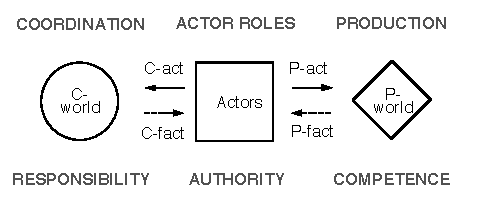
\includegraphics[width=10cm, keepaspectratio]{img/OperationAxiom}
    \caption{The operation axiom\todo{citation}}
    \label{fig:OperationAxiom}
\end{figure}

By performing production acts (P-acts for short) the subjects contribute to bringing about the goods and/or services that are delivered to the environment of the organization. The results of P-acts are production facts (P-facts for short), which can be divided into material (something is manufactured, stored or transported) and immaterial (decisions or judgements) facts.

By performing coordination acts (C-acts for short) subjects enter into and comply with commitments towards each other regarding the performance of production acts. A C-act is performed by one actor, the performer, and directed to another actor, the addressee. C-acts consist of an intention (e.g. request, promise, question, assertion) and a proposition (the performer proclaims the fact and the associated time the intention is about) and result in coordination facts (C-facts for short).

The \textbf{transaction axiom} tells us that C-acts are performed as steps in universal patterns, called transactions. This axiom reveals universal socionomic patterns of coordination that hold for all organizations. The standard transaction pattern is shown in \cref{fig:TransactionPattern}. A white box represents a C-act type and a white disk represents a C-fact type. A gray box represents a P-act type and a gray diamond a P-fact type. 

\begin{figure}[ht!] 
	\centering
    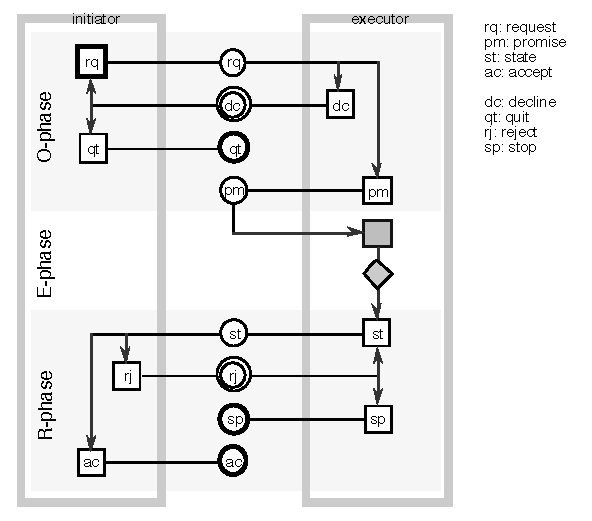
\includegraphics[width=12cm, keepaspectratio]{img/TransactionPattern}    
    \caption{The standard transaction pattern \todo{citation}}
    \label{fig:TransactionPattern}
\end{figure}

Two actors are involved in a transaction, the initiator and the executor. A transaction evolves in three phases: the order phase (O-phase for short), the execution phase (E-phase for short), and the result phase (R-phase for short).

The \textbf{composition axiom} tells us how P-facts are interrelated. It states that every transaction is enclosed in some other transaction, or is a customer transaction of the organization under consideration, or is a self-activation transaction. According to Dietz this axiom provides the basis for a well-founded definition of the notion of business process.

The \textbf{distinction axiom} (\cref{fig:DisctinctionAxiom} tells us that actors exert three basic human abilities: performa, informa, and forma. Through the distinction axiom a substantial reduction of complexity and diversity is achieved, regarding both the coordination and the production in an organization.

\begin{figure}[ht!]
	\centering
    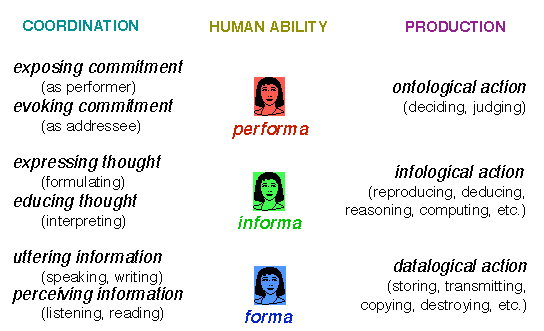
\includegraphics[width=10cm, keepaspectratio]{img/DistinctionAxiom}
    \caption{The distinction axiom\todo{citation}}
    \label{fig:DisctinctionAxiom}
\end{figure}

\subsection{The Organization Theorem}

The organization theorem combines the benefits of these axioms into one concise, comprehensive, coherent, and consistent notion of enterprise. This theorem states that the organization of an enterprise is a heterogeneous system that is constituted as the layered integration of three homogeneous systems: the B-organization (from Business), the I-organization (from Intellect), and the D-organization (from Document). Figure \ref{fig:OrganizationPyramid} visualizes the organization theorem and shows us that the D-organization supports the I-organization, which supports the B-organization. The coordination parts of these three systems are similar, they only differ in the kind of production: the production of the B-organization is ontological, the production in the I-organization is infological, and the production in the D-organization is datalogical.

\begin{figure}[ht!]
	\centering
    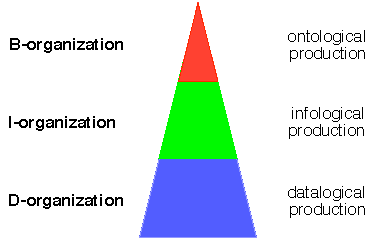
\includegraphics[width=10cm, keepaspectratio]{img/OrganizationPyramid}
    \caption{The organization theorem\todo{citation}}
    \label{fig:OrganizationPyramid}
\end{figure}
\end{quote}

\section{Modeling with DEMO}
In this section, firstly short description of modeling aspects is provided and then a illustrative example how modeling with \gls{demo} can be more precise and shorter than creating model with \gls{bpmn}. 



\subsection{Organization Construction Diagram}

\subsection{Process Structure Diagram}

